%!TEX root = ../paper.tex

The simulated datasets are a superset of a selection of the sets used by \textcite{ferdosi2011comparison}. \Cref{fig:3:simulated:datasets} shows scatter plots of these sets, their definition is given in \cref{tab:3:simulated:datasets}.

\begin{figure*}
	\centering
	\beforeFinalVersion{Remove ticks and labels.}
	\beforeFinalVersion{Fix the length of the axis of dataset \baakmanTwoNum.}
	%!TEX root = ../paper.tex
%Ferdosi Sets 1
\begin{subfigure}{0.23\textwidth}
	\centering
	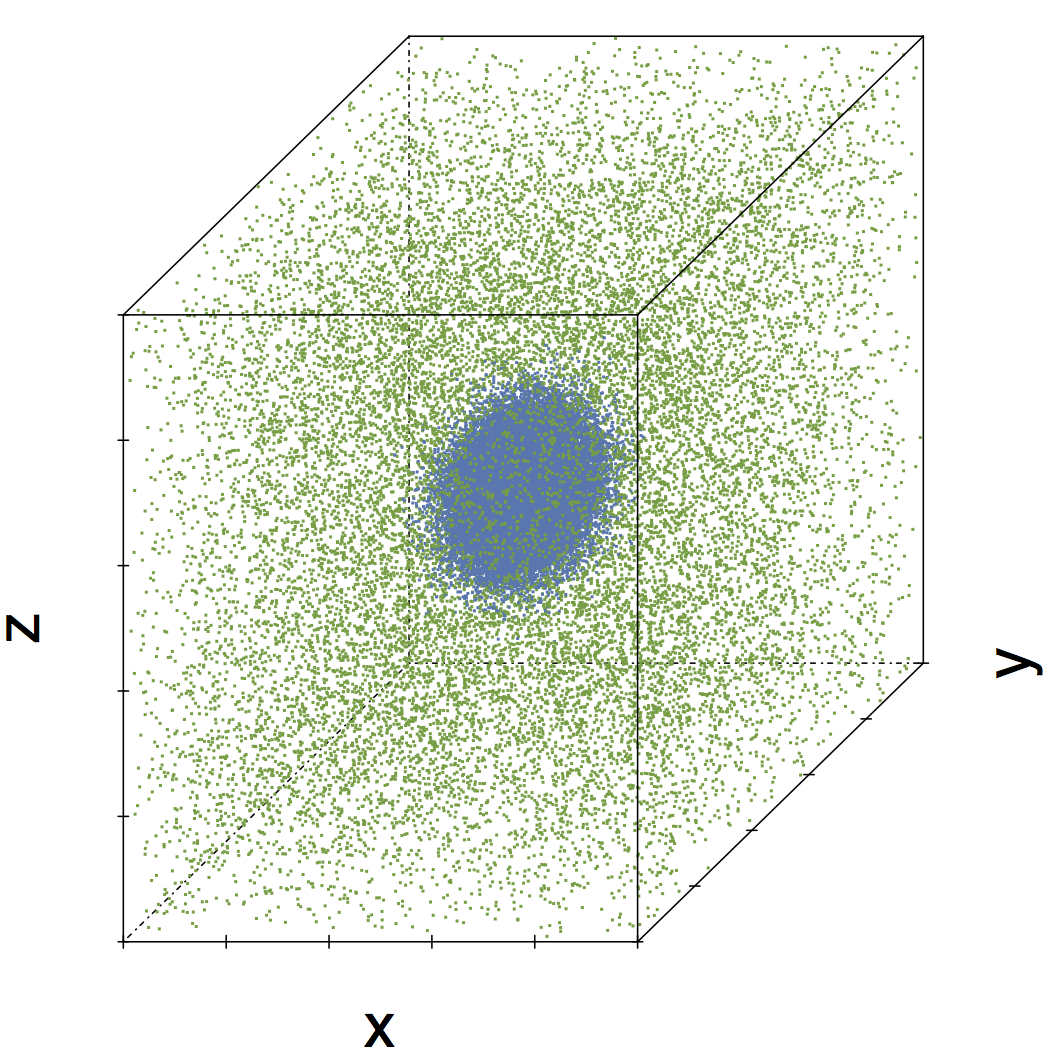
\includegraphics[width=\textwidth]{3/img/datasetplot_ferdosi_1_60000.png}
	\caption{Set \ferdosiOne}
	\label{fig:3:simulated:datasets:ferdosi1}
\end{subfigure}
% Baakman 1	
\begin{subfigure}{0.23\textwidth}
	\centering
	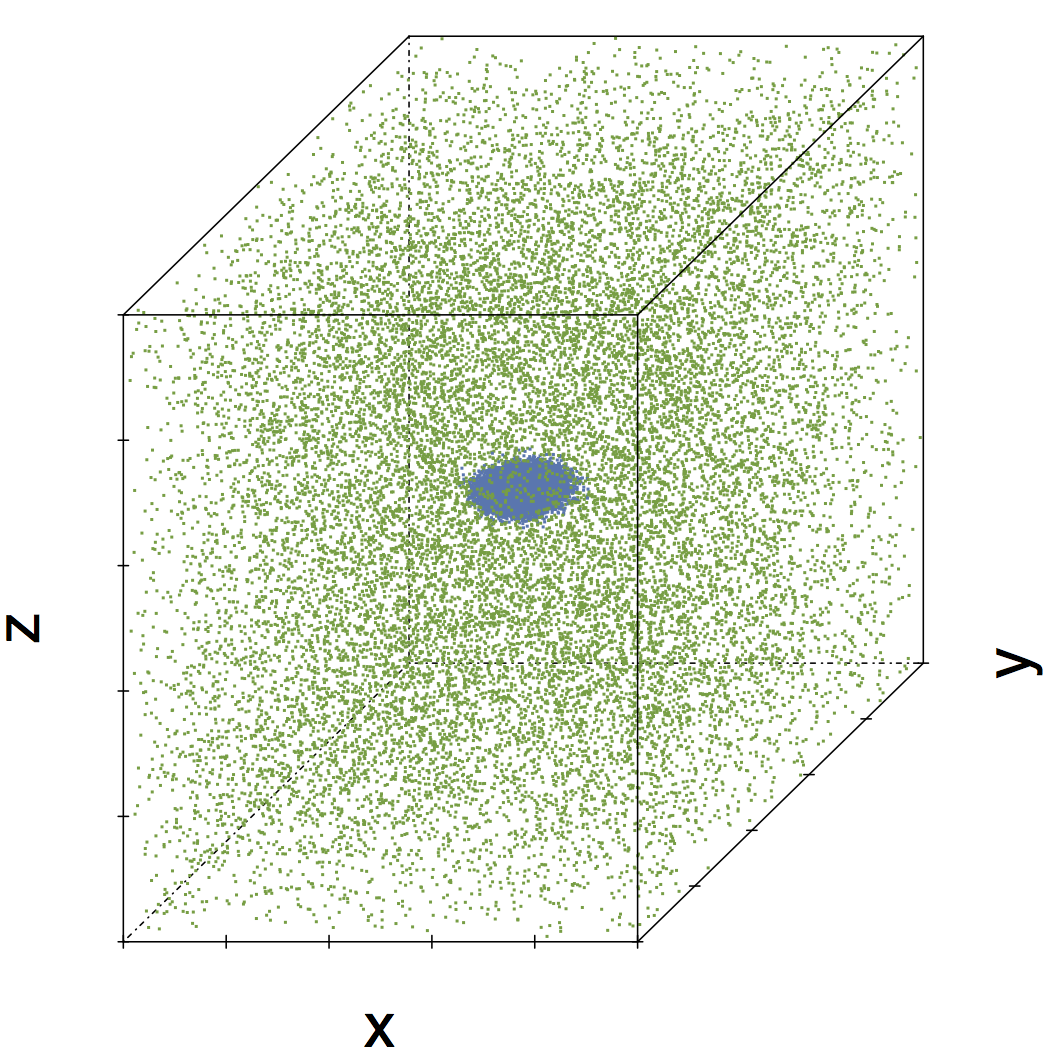
\includegraphics[width=\textwidth]{3/img/datasetplot_baakman_1_60000.png}
	\caption{Set \baakmanOne}
	\label{fig:3:simulated:datasets:baakman1}
\end{subfigure}
% Baakman 4
\begin{subfigure}{0.23\textwidth}
	\centering
	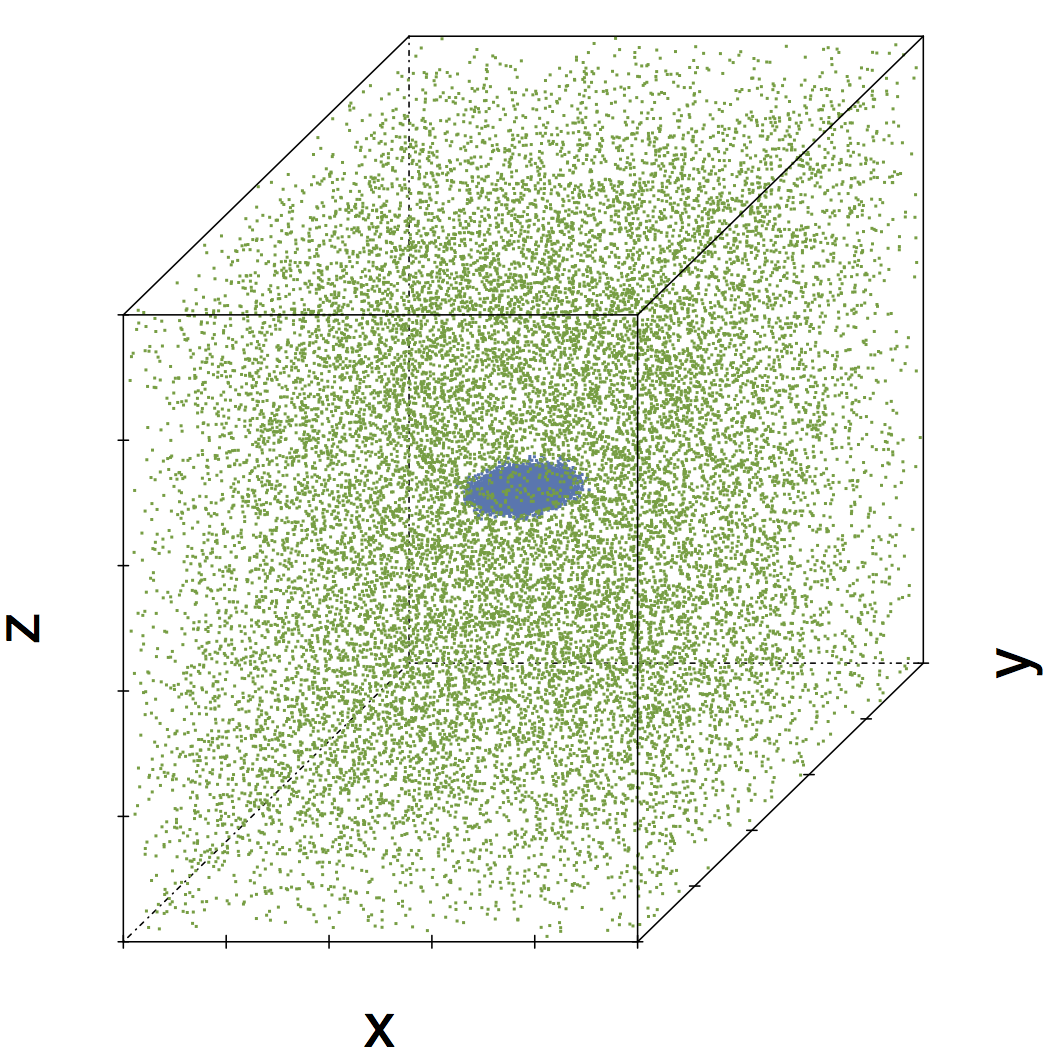
\includegraphics[width=\textwidth]{3/img/datasetplot_baakman_4_60000.png}
	\caption{Set \baakmanFour}
	\label{fig:3:simulated:datasets:baakman4}
\end{subfigure}	
% Baakman 5
\begin{subfigure}{0.23\textwidth}
	\centering
	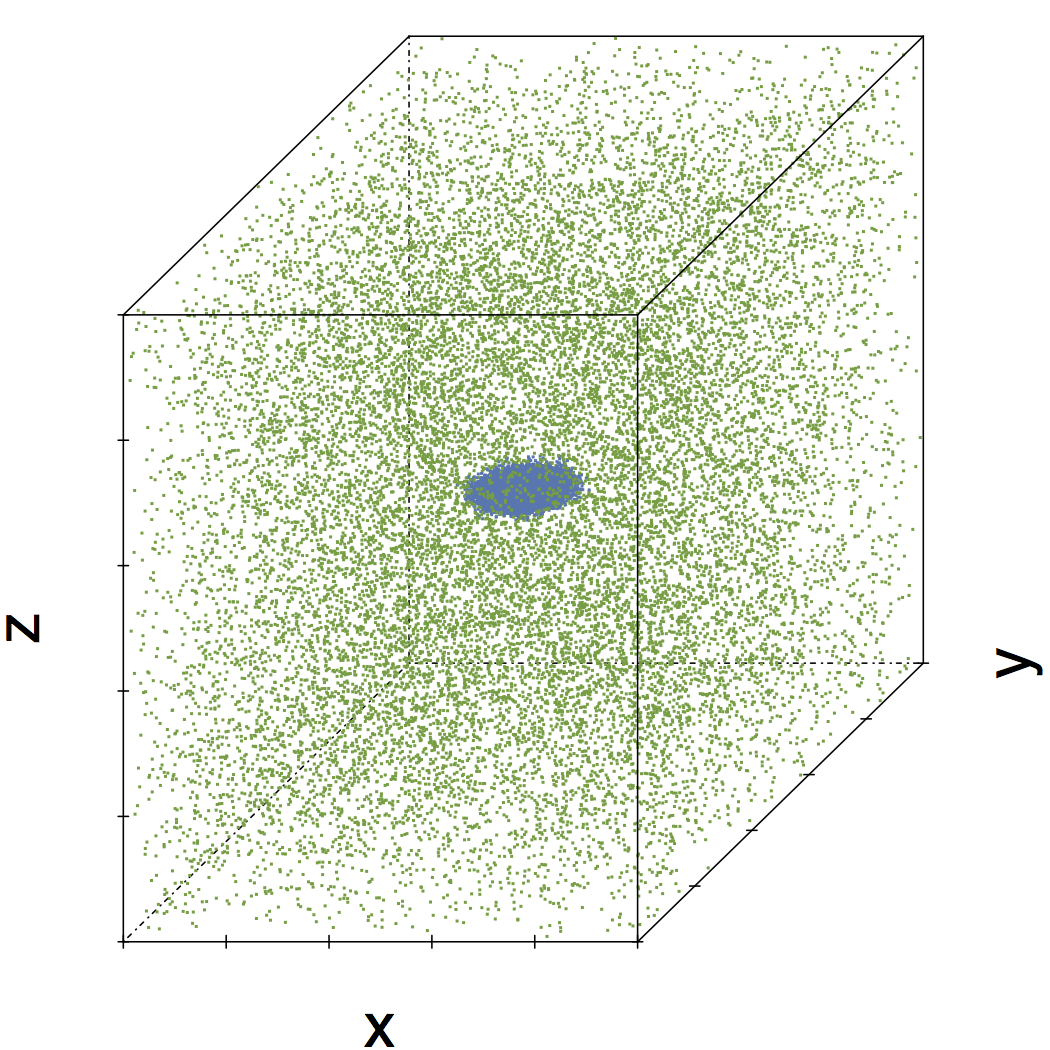
\includegraphics[width=\textwidth]{3/img/datasetplot_baakman_5_60000.png}
	\caption{Set \baakmanFive}
	\label{fig:3:simulated:datasets:baakman5}
\end{subfigure}	
% Ferdosi Set 2
\begin{subfigure}{0.23\textwidth}
	\centering
	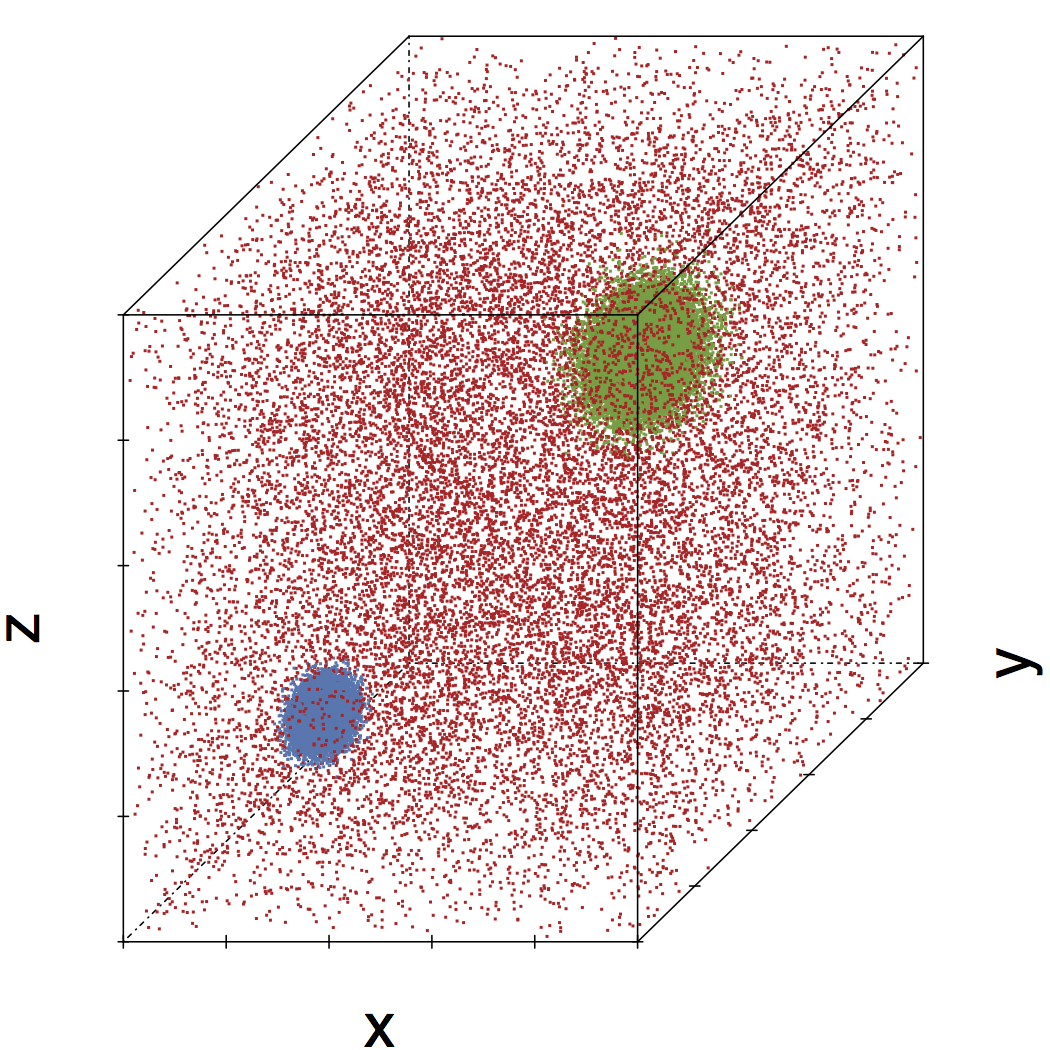
\includegraphics[width=\textwidth]{3/img/datasetplot_ferdosi_2_60000.png}
	\caption{Set \ferdosiTwo}
	\label{fig:3:simulated:datasets:ferdosi2}
\end{subfigure}	
% Baakman 2
\begin{subfigure}{0.23\textwidth}
	\centering
	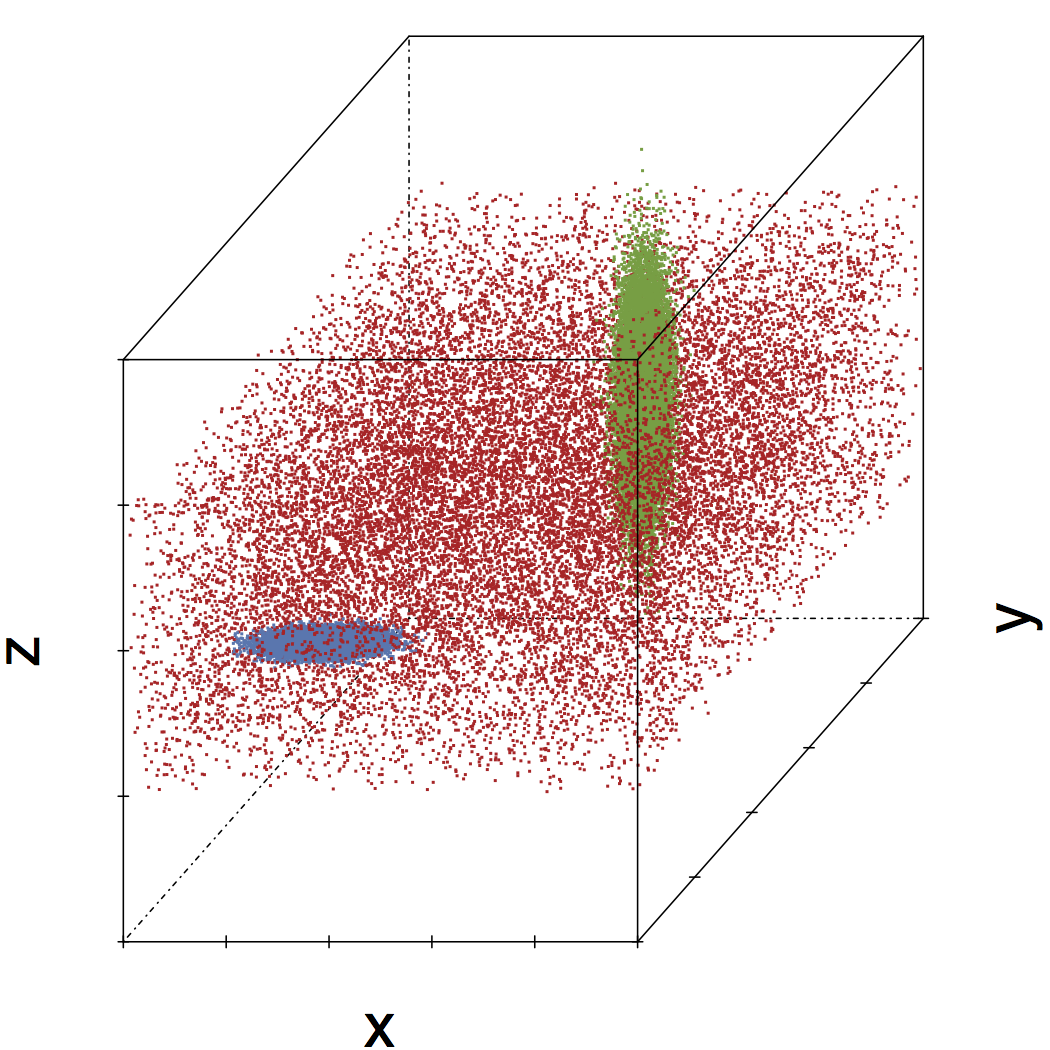
\includegraphics[width=\textwidth]{3/img/datasetplot_baakman_2_60000.png}
	\caption{Set \baakmanTwo}
	\label{fig:3:simulated:datasets:baakman2}
\end{subfigure}	
% Ferdosi Set 3
\begin{subfigure}{0.23\textwidth}
	\centering
	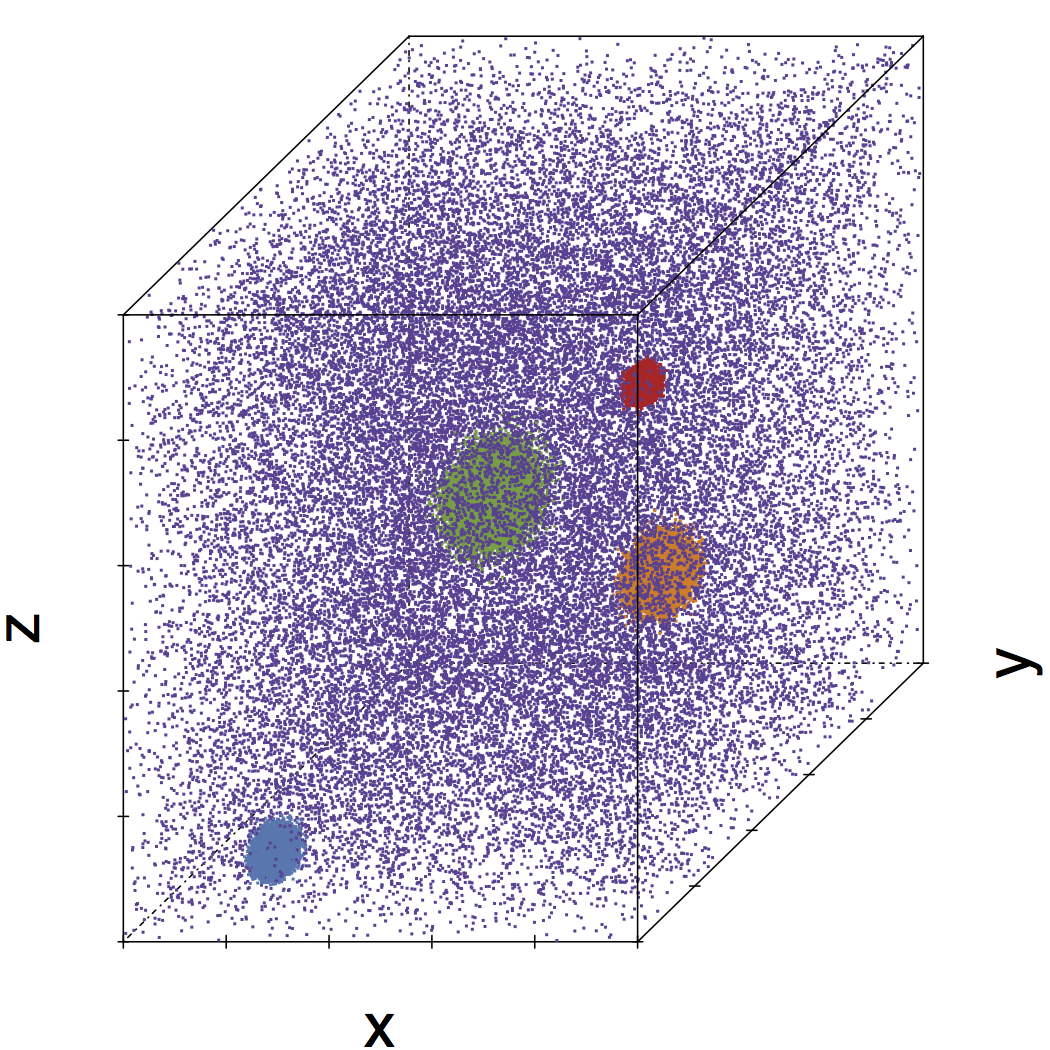
\includegraphics[width=\textwidth]{3/img/datasetplot_ferdosi_3_120000.png}
	\caption{Set \ferdosiThree}
	\label{fig:3:simulated:datasets:ferdosi3}
\end{subfigure}			
% Baakman 3
\begin{subfigure}{0.23\textwidth}
	\centering
	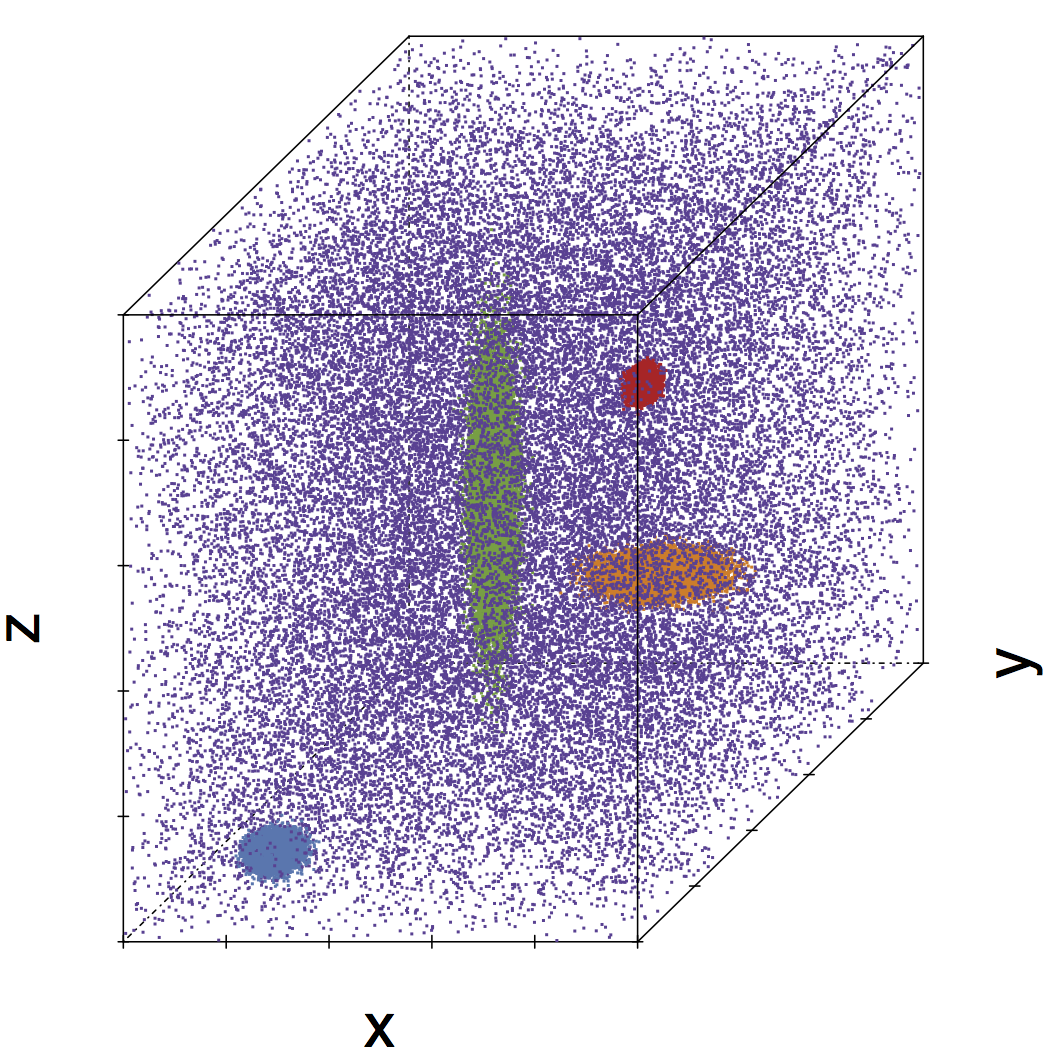
\includegraphics[width=\textwidth]{3/img/datasetplot_baakman_3_120000.png}
	\caption{Set \baakmanThree}
	\label{fig:3:simulated:datasets:baakman3}
\end{subfigure}
	\caption{Scatter plot representation of the datasets defined in \cref{tab:3:simulated:datasets}. The colors of the different components correspond to the colors used in \cref{tab:3:simulated:datasets}.}
	\label{fig:3:simulated:datasets}
\end{figure*}

\begin{table*}[!htbp]
	\centering
	%!TEX root = ../paper.tex

\begin{tabular}{@{}cclS[table-format=+1.1e+1,scientific-notation=true,round-mode=places,round-precision=1]l@{}}
\toprule
Set 			&~						& Component					& {Number} 	& Distribution\\
\midrule
% Ferdosi 1
\ferdosiOne 	&\legendComponentOne		& Trivariate Gaussian 		& 40000		& $(x, y, z) \sim \gaussDist{[50, 50, 50]}{\diag(30)}$\\
~ 				&\legendComponentNoise	& Uniform random background	& 20000		& $(x, y, z) \sim \uniformDist{[0, 0, 0]}{[100, 100, 100]}$\\
% Ferdosi 2
\hline
\ferdosiTwo 	&\legendComponentOne	& Trivariate Gaussian 1		& 20000		& $(x, y, z) \sim \gaussDist{[25, 25, 25]}{\diag(5)}$\\
~ 				&\legendComponentTwo	& Trivariate Gaussian 2		& 20000		& $(x, y, z) \sim \gaussDist{[65, 65, 65]}{\diag(20)}$\\
~ 				&\legendComponentNoise	& Uniform random background	& 20000		& $(x, y, z) \sim \uniformDist{[0, 0, 0]}{[100, 100, 100]}$\\
% Ferdosi 3
\hline
\ferdosiThree	&\legendComponentOne 	& Trivariate Gaussian 1 	& 20000		& $(x, y, z) \sim \gaussDist{[24, 10, 10]}{\diag(2)}$\\
~ 				&\legendComponentTwo	& Trivariate Gaussian 2 	& 20000		& $(x, y, z) \sim \gaussDist{[33, 70, 40]}{\diag(10)}$\\
~ 				&\legendComponentThree	& Trivariate Gaussian 3 	& 20000		& $(x, y, z) \sim \gaussDist{[90, 20, 80]}{\diag(1)}$\\
~ 				&\legendComponentFour	& Trivariate Gaussian 4 	& 20000		& $(x, y, z) \sim \gaussDist{[60, 80, 23]}{\diag(5)}$\\
~ 				&\legendComponentNoise	& Uniform random background	& 40000		& $(x, y, z) \sim \uniformDist{[0, 0, 0]}{[100, 100, 100]}$\\
% Baakman 1
\hline
\baakmanOne		&\legendComponentOne	& Trivariate Gaussian 		& 40000		& $(x, y, z) \sim \gaussDist{[50, 50, 50]}{\diag([9, \sqrt{3}, \sqrt{3}])}$\\
~ 				&\legendComponentNoise	& Uniform random background	& 20000		& $(x, y, z) \sim \uniformDist{[0, 0, 0]}{[100, 100, 100]}$\\
% Baakman 2
\hline
\baakmanTwo		&\legendComponentOne	& Trivariate Gaussian 1		& 20000		& $(x, y, z) \sim \gaussDist{[25, 25, 25]}{\diag([25, \sqrt{5}, \sqrt{5}])}$\\
~ 				&\legendComponentTwo	& Trivariate Gaussian 2		& 20000		& $(x, y, z) \sim \gaussDist{[65, 65, 65]}{\diag([\sqrt{20}, \sqrt{20}, 400])}$\\
~ 				&\legendComponentNoise	& Uniform random background	& 20000		& $(x, y, z) \sim \uniformDist{[0, 0, 0]}{[150, 150, 150]}$\\
% Baakman 3
\hline
\baakmanThree	&\legendComponentOne 	& Trivariate Gaussian 1 	& 20000		& $(x, y, z) \sim \gaussDist{[24, 10, 10]}{\diag([4, \sqrt{2}, \sqrt{2}])}$\\
~ 				&\legendComponentTwo	& Trivariate Gaussian 2 	& 20000		& $(x, y, z) \sim \gaussDist{[33, 70, 40]}{\diag([\sqrt{10}, \sqrt{10}, 100])}$\\
~ 				&\legendComponentThree	& Trivariate Gaussian 3 	& 20000		& $(x, y, z) \sim \gaussDist{[90, 20, 80]}{\diag(1)}$\\
~ 				&\legendComponentFour	& Trivariate Gaussian 4 	& 20000		& $(x, y, z) \sim \gaussDist{[60, 80, 23]}{\diag([25, \sqrt{5}, \sqrt{5}])}$\\
~ 				&\legendComponentNoise	& Uniform random background	& 40000		& $(x, y, z) \sim \uniformDist{[0, 0, 0]}{[100, 100, 100]}$\\
% Baakman 4
\hline
\baakmanFour	&\legendComponentOne	& Trivariate Gaussian 		& 40000		& $(x, y, z) \sim \gaussDist{[50, 50, 50]}{\diag([9, 2 * \sqrt{3}, \rfrac{1}{2} \sqrt{3}])}$\\
~ 				&\legendComponentNoise	& Uniform random background	& 20000		& $(x, y, z) \sim \uniformDist{[0, 0, 0]}{[100, 100, 100]}$\\
% Baakman 5
\hline
\baakmanFive	&\legendComponentOne	& Trivariate Gaussian 		& 40000		& $(x, y, z) \sim \gaussDist{[50, 50, 50]}{\diag([9, 3, 1])}$\\
~ 				&\legendComponentNoise	& Uniform random background	& 20000		& $(x, y, z) \sim \uniformDist{[0, 0, 0]}{[100, 100, 100]}$\\
\bottomrule
\end{tabular}
	\caption{The datasets used to test the estimators. The column `Number' indicates for each component of the dataset how many data points are sampled from that component. \gaussDist{\varMean}{\varCovarianceMatrix} denotes a Gaussian distribution with mean \varMean and covariance matrix \varCovarianceMatrix. A diagonal matrix with the values $x_1,\, \cdots,\, x_\varDim$ on the diagonal is represented as $\diag([x_1,\,\cdots,\,x_\varDim]])$, a scalar matrix with $x$ on the diagonal is shown as $\diag(x)$. \uniformDist{a}{b} denotes a uniform distribution with its minimum and maximum set to $a$ and $b$, respectively. The colors shown in the second column correspond with the colors used for these components of the data set throughout the paper.} 	
	\label{tab:3:simulated:datasets}
\end{table*}

% Ferdosi 1/3
Dataset \ferdosiOne, \ferdosiTwo, and \ferdosiThree, shown in \cref{fig:3:simulated:datasets:ferdosi1,fig:3:simulated:datasets:ferdosi3,fig:3:simulated:datasets:ferdosi2}, respectively, are taken directly from \citeauthor{ferdosi2011comparison}. They consist of a number of spherical Gaussian distributions with random noise added. The means of the Gaussian distribution are chosen in such a way that it is unlikely that the distributions overlap.

%Baakman 1/3
\Cref{fig:3:simulated:datasets:baakman1,fig:3:simulated:datasets:baakman3,fig:3:simulated:datasets:baakman2} present dataset \baakmanOne, \baakmanTwo, and \baakmanThree. These datasets are created from dataset \ferdosiOne, \ferdosiTwo and, \ferdosiThree, respectively. This is done in such a way that the volumes of the eigenspheres of the covariance matrices of the components in the derived datasets have the same volume as the eigenellipsoids of the covariance matrices of the associated components in the original dataset. Furthermore if $a$ is the eigenvalue of the original covariance matrix, the eigenvalues of the covariance matricex of the derived component are $a^2$, $\sqrt{a}$ and $\sqrt{a}$. Consequently the volumes the eigenspheres of the covariance matrices of the Gaussians in dataset \baakmanOne, \baakmanTwo and, \baakmanThree are equal to those of dataset \ferdosiOne, \ferdosiTwo and, \ferdosiThree, respectively.

% Baakman 4/5
In dataset \baakmanFour and \baakmanFive, illustrated in \cref{fig:3:simulated:datasets:baakman3,fig:3:simulated:datasets:baakman4} the semi axes of the ellipsoids all have different lengths. The largest minor axis of the Trivariate Gaussian in dataset \baakmanFour is a factor two larger than the smallest minor axis in that dataset. Whereas in dataset \baakmanFive the largest minor axis is exponentially larger than the smallest minor axis. 

%Expectations for the datasets
% Ferdosi 1/3
We expect the MBE and shape-adaptive MBE to perform comparable on dataset \ferdosiOne through \ferdosiThree, as other than the randomly sampled noise these sets only contain data sampled from a Gaussian distribution with a diagonal covariance matrix. Which results in an equal spread of the data in all dimensions for the non-noise data. 
% Baakman 1/5
Given the elongated shape of the non-noise components in dataset \baakmanOne, \baakmanTwo, \baakmanThree, \baakmanFour, and \baakmanFive we hypothesize that the shape-adaptive estimator outperforms the estimator that is not shape adaptive.

%Conclusion
The datasets with a single Gaussian which are increasingly more elongated, \ie dataset \ferdosiOne, \baakmanOne, \baakmanFour and, \baakmanFive, allow us to investigate the influence of the ellipitcalness on the performance of the estimators. Whereas the datasets with multiple ellipsoids, \ie dataset \ferdosiTwo, \ferdosiThree, \baakmanTwo, and \baakmanThree, make it possible to investigate the performance of the classifier on more complex density fields that better approximate real world data. 